\begin{normalsize}

\subsection{Доказательство теоремы}

\begin{lemma}
    Зафиксируем $k, c \in \N$ с $k \geq 3$. Предположим, что $\forall c'$ верна VDW$(k-1, c')$. Тогда $\forall r: \exists U = U(r)$, такое что для любой $c$-раскраски $\chi: \{1, \ldots, |U|\} \to \{1, \ldots, c\}$ верно одно из следующих утверждений:

    \begin{enumerate}
        \item $\exists a, d$, такие что $\chi(a) = \chi(a + d) = \cdots = \chi(a + (k - 1)d)$.
        
        \item $\exists a, d_1, \ldots, d_r$, такие что:
        \begin{gather*}
            \chi(a + d_1) = \chi(a + 2d_1) = \cdots = \chi(a + (k - 1)d_1)\\
            \chi(a + d_2) = \chi(a + 2d_2) = \cdots = \chi(a + (k - 1)d_2)\\
            \vdots\\
            \chi(a + d_r) = \chi(a + 2d_r) = \cdots = \chi(a + (k - 1)d_r)
        \end{gather*}
        и $\forall i \neq j: \chi(a + d_i) \neq \chi(a + d_j)$.
    \end{enumerate}

    Неформально: в $c$-раскраске достаточно большого начального отрезка $\N$ найдется либо одноцветная $k$-а.п., либо сколь угодно большое число одноцветных $(k - 1)$-а.п. с общим началом. При $c + 1$ штук прогрессий второе невозможно, то есть верно первое.

\end{lemma}

\begin{proof}

    $U(r): min U$, такое что лемма верна(минимальная длина блока для леммы, где существует $(k - 1)$-а.п. для $r$ цветов, и есть общий элемент)

    Покажем верхнюю границу на $U(r) \implies U(r)$ существует.
    
    \textsl{База:} $r = 1$. 

    Покажем, что $U(1) \leq 2W(k - 1, c)$.

    Пусть $\chi: \{1, \ldots, 2W(k-1, c)\} \to \{1, \ldots, c\}$.

    Применим VDW$(k - 1, c)$ ко второй половине $\{1, \ldots, U(1)\}$, чтобы получить $a, d \in N$, такие что 

    \[ \chi(a + d) = \chi(a + 2d) = \cdots = \chi(a + (k - 1)d) \]

    и $a \in \{1, \ldots, U(1)\}$.

    \begin{center}
        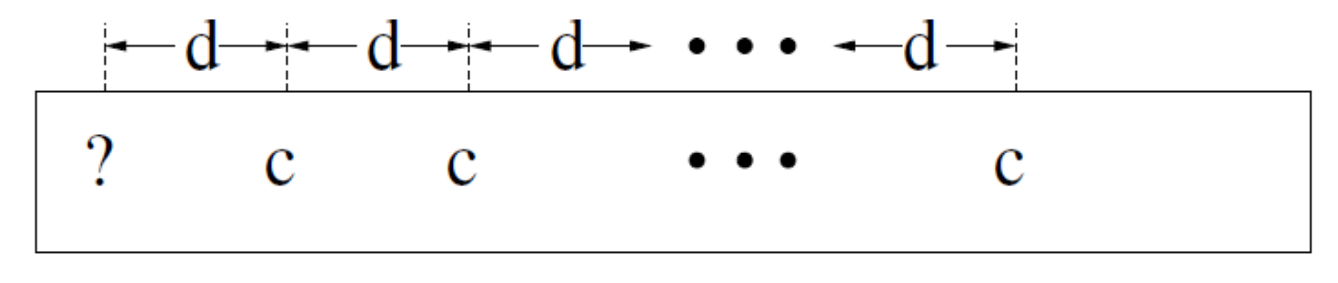
\includegraphics[width=0.7\textwidth]{par51vdwlemma.png}
    \end{center}

    \begin{itemize}
        \item Если $\chi(a) = \chi(a + d)$, то $a, a + d, \ldots, a + (k - 1)d$ является одноцветной $k$-а.п., то есть выполняется первое утверждение.
        
        \item Если $\chi(a) \neq \chi(a + d)$, то выполняется второе утверждение.
    \end{itemize}
    
    \textsl{Переход:} Пусть $U(r)$ существует. Докажем, что $U(r + 1) \leq 2U(r) \cdot W(k - 1, c^{U(r)})$.

    Пусть $\chi: \{1, \ldots, U\} \to \{1, \ldots, c\}$

    Рассмотрим $\{1, \ldots, U\}$ как $U(r) \cdot W(k - 1, c^{U(r)})$ чисел, за которыми следуют $W(k - 1, c^{U(r)})$ блоков размера $U(r)$.

    Обозначим эти блоки $B_1, B_2, \ldots, B_{W(k - 1, c^{U(r)})}$.

    Один блок:

    \begin{center}
        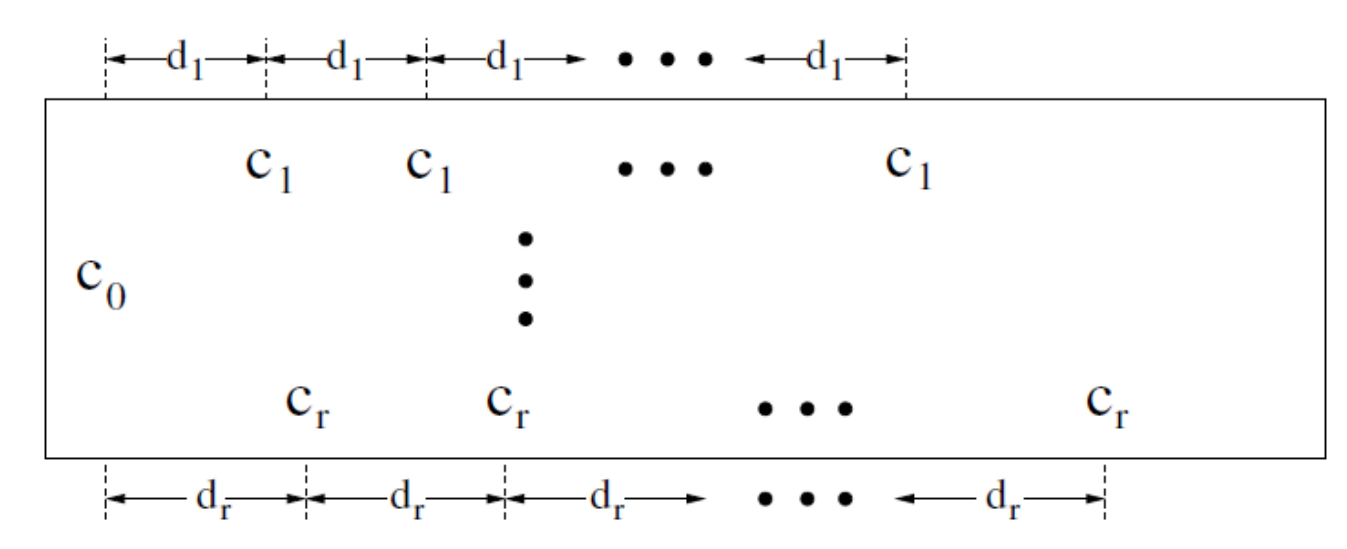
\includegraphics[width=0.7\textwidth]{par51vdwblock.png}
    \end{center}

    Рассматриваем $c$-раскраску второй половины $\{1, \ldots, U\}$ как $c^{U(r)}$-раскраску блоков (обозначим ее $\chi^*$).

    По определению $W(k - 1, c^{U(r)})$ получаем одноцветную $(k - 1)$-а.п. блоков.

    \begin{center}
        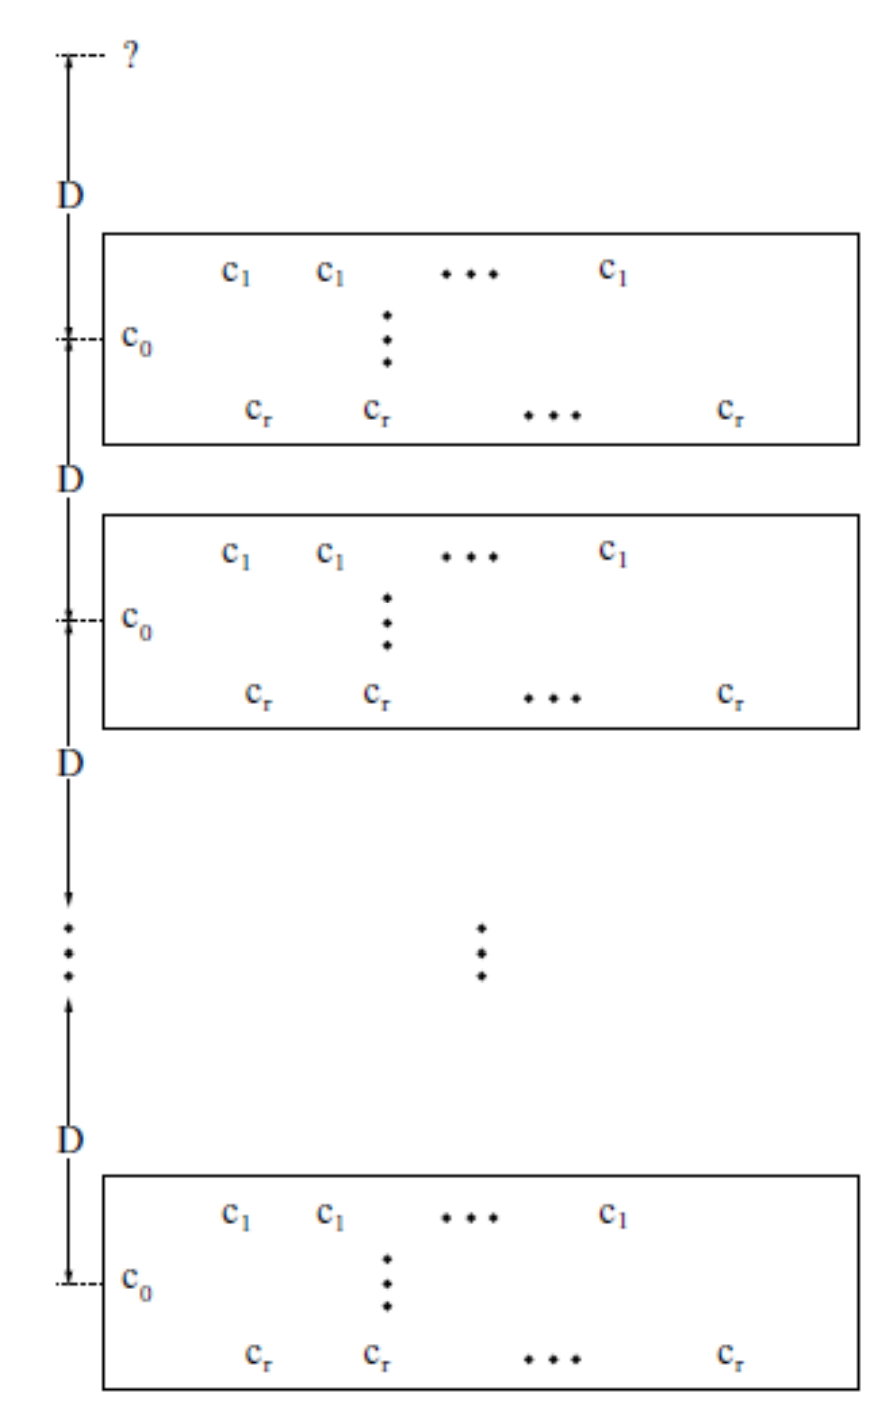
\includegraphics[width=0.6\textwidth]{par51vdw.png}
    \end{center}

    Отсюда получаем $A, D'$, такие что

    \[ \chi^*(B_A + D') = \chi^*(B_A + D') = \cdots = \chi^*(B_A + (k - 2)D') \]

    Длина блока $B_A$ равна $U(r) \implies$ применяем предположение индукции.
    
    Если верно первое утверждение, то имеем одноцветную $k$-а.п. и все доказано.

    Если верно второе утверждение, то имеем $a', d_1, d_2, d_r$, с $a' \in B_A$ и 

    \begin{gather*}
        \{ a' + d_1, a' + 2d_1, \ldots, a' + (k - 1)d_1 \} \subseteq B_A \\
        \{ a' + d_2, a' + 2d_2, \ldots, a' + (k - 1)d_2 \} \subseteq B_A \\
        \vdots \\
        \{ a' + d_r, a' + 2d_r, \ldots, a' + (k - 1)d_r \} \subseteq B_A
    \end{gather*}

    \begin{gather*}
        \chi(a' + d_1) = \chi(a' + 2d_1) = \cdots = \chi(a' + (k - 1)d_1) \\
        \chi(a' + d_2) = \chi(a' + 2d_2) = \cdots = \chi(a' + (k - 1)d_2) \\
        \vdots \\
        \chi(a' + d_r) = \chi(a' + 2d_r) = \cdots = \chi(a' + (k - 1)d_r)
    \end{gather*}

    Где $\chi(a' + d_i)$ имеют разные цвета, отличные от $a'$ (иначе уже есть одноцветная $k$-а.п.).

    Так как блоки рассматриваем как точки на расстоянии $D'$, и каждый блок длины $U(r)$, то соответствующие элементы в блоках на расстоянии $D = D' \cdot U(r)$. Отсюда 

    \begin{gather*}
        \chi(a' + d_1) = \chi(a' + D + d_1) = \cdots = \chi(a' + (k - 2)D + d_1) \\
        \chi(a' + d_2) = \chi(a' + D + d_2) = \cdots = \chi(a' + (k - 2)D + d_2) \\
        \vdots \\
        \chi(a' + d_r) = \chi(a' + D + d_r) = \cdots = \chi(a' + (k - 2)D + d_r)
    \end{gather*}

    До сих пор все было внутри второй половины $\{1, \ldots, U\}$. Так как 

    \[ a' > \frac{1}{2}U = U(r) \cdot W(k - 1, c^{U(r)}) \]

    и

    \[ D \leq \frac{1}{k - 1} U(r) W(k - 1, c^{U(r)}) \leq U(r) W(k - 1, c^{U(r)}), \]

    то получаем $a = a' - D > 0 \implies a \in \{1, \ldots, U\}.~a$ будет новым общим началом а.п.

    \begin{gather*}
        \chi(a + D + d_1) = \chi(a + 2(D + d_1)) = \cdots = \chi(a + (k - 1)(D + d_1))\\
        \chi(a + D + d_2) = \chi(a + 2(D + d_2)) = \cdots = \chi(a + (k - 1)(D + d_2))\\
        \vdots \\
        \chi(a + D + d_r) = \chi(a + 2(D + d_r)) = \cdots = \chi(a + (k - 1)(D + d_r))
    \end{gather*}

    где цвета всех прогрессий различны.

    Нам нужна $(r + 1)$-ая прогрессия.

    Рассмотрим $\{a + D, a + 2D, \ldots, a + (k - 1)d\}$.

    Все эти точки одноцветны (так как внутри одинаково окрашенных блоков).

    И так как $\forall i: \chi(a') \neq \chi(a' + d_i)$, то цвет новой прогрессии отличается от $r$ предыдущих.

    То есть имеем $r + 1$ одноцветных $(k - 1)$-а.п., все разных цветов, с общим продолжением $a$. Новые параметры $a, D + d_1, \ldots, D + d_r, D$.

\end{proof}

\begin{proof} [ теоремы Ван-дер-Вардена]
    
    Индукция по $k$.

    \textbf{База:} $W(1, c) = 1$.

    \textbf{Индукция:} Предположим, что верно VDW$(k - 1, c)$.

    По лемме при $r = c$ в любой $c$-раскраске $\{1, \ldots, U(c)\}$ либо есть одноцветная $k$-а.п., либо есть $c$ одноцветных $(k - 1)$-а.п., которые все раскрашены разными цветами, и число $a$, которое окрашено в цвет, отлиный от цветов а.п. 

    Так как всего имеется только $c$ цветов, то мы должны получить одноцветную $k$-а.п. Отсюда $W(k, c) \leq U(c)$ и, следовательно, оно существует.

\end{proof}

\subsubsection*{Верхние границы на числа Ван дер Вардена}

То, что получается из доказательства --- аккермановская функция.

\begin{exerc}
    Получить в явном виде оценци из доказательства теоремы.
\end{exerc}

\begin{theorem} [Gowers, 2001]
    \[ W(k, c) \leq 2^{ 2^{ c^{ 2^{ 2^{ k + 9}}}}}. \]
\end{theorem}

\begin{notice}
    Грэхэм: 1000\$ за доказательство $W(k, 2) \leq 2^{ k^2 }$.
\end{notice}

\end{normalsize}